% Copyright (C) 2012 Shi.Zhan <g.shizhan.g@gmail.com>
%
% Permission is hereby granted, free of charge, to any person obtaining a copy of this software and associated documentation files (the "Software"), to deal in the Software without restriction, including without limitation the rights to use, copy, modify, merge, publish, distribute, sublicense, and/or sell copies of the Software, and to permit persons to whom the Software is furnished to do so, subject to the following conditions:
%
% The above copyright notice and this permission notice shall be included in all copies or substantial portions of the Software.
%
% THE SOFTWARE IS PROVIDED "AS IS", WITHOUT WARRANTY OF ANY KIND, EXPRESS OR IMPLIED, INCLUDING BUT NOT LIMITED TO THE WARRANTIES OF MERCHANTABILITY, FITNESS FOR A PARTICULAR PURPOSE AND NONINFRINGEMENT. IN NO EVENT SHALL THE AUTHORS OR COPYRIGHT HOLDERS BE LIABLE FOR ANY CLAIM, DAMAGES OR OTHER LIABILITY, WHETHER IN AN ACTION OF CONTRACT, TORT OR OTHERWISE, ARISING FROM, OUT OF OR IN CONNECTION WITH THE SOFTWARE OR THE USE OR OTHER DEALINGS IN THE SOFTWARE.
%
% 课程:人机交互技术及应用
% 班级:传播学1001班
% 课时:40学时,2012年秋季1~10周,每周一、三
% 地点:东九楼D212
% 主页:http://code.google.com/p/hci-course/
% 教师:施展 
% 单位:华中科技大学 武汉光电国家实验室
%
\documentclass{beamer}
\usepackage{fontspec,xunicode,xltxtra,beamerthemesplit}
%\usetheme{Hannover} % White background
\usetheme{Berkeley} % Blue background
\setmainfont[
	BoldFont={WenQuanYi Zen Hei},
	ItalicFont={WenQuanYi Micro Hei}
]{WenQuanYi Micro Hei}
\setsansfont[
	BoldFont={WenQuanYi Zen Hei},
	ItalicFont={WenQuanYi Micro Hei}
]{WenQuanYi Micro Hei}

% 中文环境自动换行
\XeTeXlinebreaklocale "zh"
\XeTeXlinebreakskip = 0pt plus 1pt

% 中文环境修正导航栏
\makeatletter
\def\beamer@linkspace#1{
	\begin{pgfpicture}{0pt}{-1.5pt}{#1}{5.5pt}
		\pgfsetfillopacity{0}
		\pgftext[x=0pt,y=-1.5pt]{.}
		\pgftext[x=#1,y=5.5pt]{.}
	\end{pgfpicture}
}
\makeatother

% diagrams
\usepackage{tikz}
\usetikzlibrary{arrows,shapes}

% full page image
\newcommand{\fullPageImage}[2]{
	{
		\usebackgroundtemplate{\includegraphics[width=\paperwidth, height=\paperheight]{#1}}
		\frame[plain]{#2}
	}
}

\title{人机交互技术}
\author{施展}
\institute{华中科技大学~武汉光电国家实验室}
\date{\today}
\titlegraphic{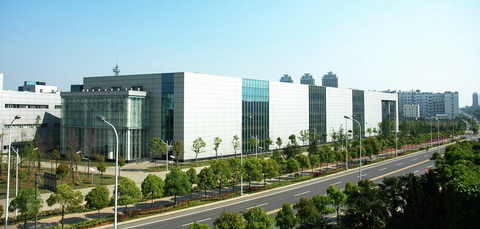
\includegraphics[width=2cm]{images/wnlo.jpg}}

\begin{document}

\begin{frame}
	\titlepage
\end{frame}

\begin{frame}
	\frametitle{内容提要}
	\tableofcontents
\end{frame}

\section{第五讲}
\begin{frame}
	\frametitle{第五讲 界面设计}
	\begin{itemize}
		\item 掌握图形用户界面的主要思想和设计的一般原则。
		\item 了解用户、用户体验、用户交互分析以及设计流程。
		\item 掌握任务分析方法方法
		\begin{itemize}
			\item 重点掌握:使用行为分析、顺序分析、协作关系分析。
		\end{itemize}
%		\item 掌握以用户为中心的界面设计方法。
	\end{itemize}
\end{frame}

\subsection{界面设计原则}
\begin{frame}
	\frametitle{界面设计原则}
	\begin{itemize}
		\item 根据表现形式,用户界面分为
		\begin{itemize}
			\item 命令行界面 \textit{Command Line Interface}
			\item 图形界面 \textit{Graphic User Interface}
			\item 多通道用户界面 \textit{Multimodal User Interface}
		\end{itemize}
	\end{itemize}
\end{frame}

\begin{frame}
	\frametitle{图形用户界面的主要思想}
	\begin{itemize}
		\item 图形用户界面的三个重要思想
		\begin{itemize}
			\item 桌面隐喻\\\textit{desktop metaphor}
			\item 所见即所得\\\textit{What You See Is What You Get, WYSIWYG}
			\item 直接操纵\\\textit{Direct manipulation}
		\end{itemize}
	\end{itemize}
\end{frame}

\begin{frame}
	\frametitle{桌面隐喻~\textit{desktop metaphor}}
	\beamertemplatetransparentcovereddynamicmedium
	\begin{beamerboxesrounded}[shadow=true]{桌面隐喻}
		在用户界面中用人们熟悉的桌面上的图例清楚地表示计算机可以处理的能力。
		\begin{itemize}
			\item 图形具有一定的文化和语言独立性,可以提高搜索目标的效率。
			\item 图形用户界面中的图例可以代表对象、动作、属性或其他概念。
		\end{itemize}
	\end{beamerboxesrounded}
	\pause
	\begin{beamerboxesrounded}[shadow=true]{表达方式}
		图例和文字
		\begin{itemize}
			\item 文字适用于表达某些抽象概念。
			\item 图例更易于识别,占用较少屏幕空间,可独立于语言。
		\end{itemize}
	\end{beamerboxesrounded}
\end{frame}

\begin{frame}
	\frametitle{隐喻的表现方法}
	\begin{itemize}
		\item 静态图标
		\item 动画
		\item 视频
	\end{itemize}
\end{frame}

\begin{frame}
	\frametitle{隐喻的分类}
	\begin{itemize}
		\item 直接隐喻:隐喻本身就带有操纵的对象
		\begin{itemize}
			\item 如Word中的表格、图表等图标,图标分别代表了操纵对象。
		\end{itemize}
		\item 工具隐喻:代表所使用的工具
		\begin{itemize}
			\item 如用磁盘图标隐喻存盘操作、用打印机图标隐喻打印操作等,这种隐喻设计简单、形象直观,应用也最为普遍。
		\end{itemize}
		\item 过程隐喻:通过描述操作的过程来暗示该操作
		\begin{itemize}
			\item 如Word中的撤销和恢复图标。
		\end{itemize}
	\end{itemize}
\end{frame}

\fullPageImage{images/redcons-fullpreview1-600x356.jpg}{}

\begin{frame}
	\frametitle{所见即所得}
	\beamertemplatetransparentcovereddynamicmedium
	\begin{itemize}[<+->]
		\item 在WYSIWYG交互界面中显示的用户交互行为与应用程序最终产生的结果是一致的。 
		\item 非WYSIWYG的编辑器,用户只能看到文本的控制代码,对于最后的输出结果缺乏直观的认识。
		\item 思考:孰优孰劣?
	\end{itemize}
\end{frame}

\begin{frame}
	\frametitle{WYSIWYG的弊端}
	\beamertemplatetransparentcovereddynamicmedium
	\begin{itemize}[<+->]
		\item 平台兼容
		\begin{itemize}
			\item 如果屏幕的空间或颜色的配置方案与硬件设备所提供的配置不一样,在两者之间就很难产生正确的匹配。
		\end{itemize}
		\item 结构隐藏
		\begin{itemize}
			\item 文本处理器都提供了定义章、节、小节等的标记,这些标记显式地标明了对象的属性,但并不是用户最终输出结果的一部分。
		\end{itemize}
	\end{itemize}
\end{frame}

\fullPageImage{images/texmakertop_big.jpg}{}

\begin{frame}
	\frametitle{直接操纵}
	\beamertemplatetransparentcovereddynamicmedium
	\begin{beamerboxesrounded}[shadow=true]{直接操纵}
	把操作的对象、属性、关系显式地表示出来,用光笔、鼠标、触摸屏或数据手套等指点设备直接从屏幕上获取形象化命令与数据的过程。
	\end{beamerboxesrounded}
	\pause
	\begin{beamerboxesrounded}[shadow=true]{直接操纵的对象}
	命令、数据或是对数据的某种操作。
	\end{beamerboxesrounded}
\end{frame}

\begin{frame}
	\frametitle{直接操纵的特性}
	\beamertemplatetransparentcovereddynamicmedium
	\begin{itemize}[<+->]
		\item 直接操纵的对象是动作或数据的形象隐喻
		\begin{itemize}
			\item 形象隐喻与实际内容相近,使用户能通过屏幕上的隐喻直接想象或感知其内容。
		\end{itemize}
		\item 用指点和选择代替键盘输入
		\begin{itemize}
			\item 优点:操作简便,速度快捷。
			\item 再考虑一下? % 为什么还需要键盘快捷键
		\end{itemize}
		\item 操作结果立即可见
		\begin{itemize}
			\item 用户可以及时修正操作,逐步往正确的方向前进。
		\end{itemize}
		\item 支持逆向操作
		\begin{itemize}
			\item 用户在使用系统的过程中,不可避免地会出现一些操作错误,通过逆向操作,用户可以很方便地恢复到出现错误之前的状态。
		\end{itemize}
	\end{itemize}
\end{frame}

\begin{frame}
	\frametitle{直接操纵的优缺点}
	\beamertemplatetransparentcovereddynamicmedium
	\begin{itemize}[<+->]
		\item 优点
		\begin{itemize}
			\item 借助物理的、空间的或形象的表示,而不是单纯的文字或数字的表示。依赖于视觉和手动控制的参与,可以直接操作,有利于解决问题和进行学习。
		\end{itemize}
		\item 缺点
		\begin{itemize}
			\item 与命令语言界面的某些优点相比
			\begin{itemize}
				\item 从用户界面设计者角度看,设计图形比较繁琐,需进行大量的测试和实验。
				\item \dots 快捷性再考虑
			\end{itemize}
			\item 表示复杂语义、抽象语义比较困难。
			\begin{itemize}
				\item \dots “宏”、“脚本”的意义
			\end{itemize}
		\end{itemize}
	\end{itemize}
\end{frame}

\begin{frame}
	\frametitle{图形用户界面~{\small 一般性原则}}
	\beamertemplatetransparentcovereddynamicmedium
	\begin{itemize}[<+->]
		\item 界面要具有一致性
		\begin{itemize}
			\item 在同一用户界面中,所有的菜单选择、命令输入、数据显示和其他功能应保持风格的一致性。
		\end{itemize}
		\item 常用操作要有快捷方式
		\begin{itemize}
			\item 不仅会提高用户的工作效率,还使界面在功能实现上简洁而高效。
		\end{itemize}
		\item 提供简单的错误处理
		\begin{itemize}
			\item 在出现错误时,系统应该能检测出错误,并且提供简单和容易理解的错误处理功能
		\end{itemize}
		\item 对操作人员的重要操作要有信息反馈
		\begin{itemize}
			\item 尤其是对不常用操作、至关重要操作要有信息反馈。
		\end{itemize}
	\end{itemize}
\end{frame}

\begin{frame}
	\frametitle{图形用户界面~{\small 一般性原则}}
	\beamertemplatetransparentcovereddynamicmedium
	\begin{itemize}[<+->]
		\item 操作可逆
		\begin{itemize}
			\item 对大多数动作应允许恢复(UNDO),对用户出错采取比较宽容的态度。
		\end{itemize}
		\item 设计良好的联机帮助
		\begin{itemize}
			\item 人机界面应该提供上下文敏感的求助系统,让用户及时获得帮助,尽量用简短的动词和动词短语提示命令。
		\end{itemize}
		\item 合理划分并高效地使用显示屏
		\begin{itemize}
			\item 只显示与上下文有关的信息,允许用户对可视环境进行维护,如放大、缩小窗口;
			\item 用窗口分隔不同种类的信息,只显示有意义的出错信息。
		\end{itemize}
		\item 保证信息显示方式与数据输入方式的协调一致,尽量减少用户输入的动作
		\begin{itemize}
			\item 隐藏当前状态下不可用的命令,允许用户自选输入方式,能够删除错误的输入,允许用户控制交互过程。
		\end{itemize}
	\end{itemize}
\end{frame}

\subsection{理解用户}
\begin{frame}
	\frametitle{理解用户}
	\beamertemplatetransparentcovereddynamicmedium
	\begin{itemize}[<+->]
		\item 用户是使用某种产品的人,其包含两层含义:
		\begin{itemize}
			\item 1) 用户是人类的一部分; 2) 用户是产品的使用者。
		\end{itemize}
		\item 衡量一个以用户为中心的设计的好坏,关键点是强调产品的最终使用者与产品之间的交互质量
		\begin{itemize}
			\item {\tiny 产品在特定使用环境下为特定用户用于特定用途时所具有的}有效性 Effectiveness、效率 Efficiency 和用户主观满意度 Satisfaction~\cite{iso19989241}。
		\end{itemize}
		\item 以用户为中心的设计,宗旨就是:
		\begin{itemize}
			\item {\tiny 在软件开发过程中要紧紧围绕用户,在系统设计和测试过程中,}要有用户的参与,{\tiny 以便及时获得用户的反馈信息;}
			\item {\tiny 根据用户的需求和反馈信息,}不断改进设计——迭代,{\tiny 直到满足了用户的需求,这个过程才终止。}
		\end{itemize}
	\end{itemize}
\end{frame}

% http://www.neospot.se/usability-vs-user-experience/
\fullPageImage{images/usability-vs-user-experience.jpg}{}
% By this definition Usability is a subset of the overall User Experience. Usability answers the question, "Can the user accomplish their goal?" with effectiveness, efficiency, and satisfaction about the results (as per the ISO 9241-11 definition of usability). User Experience also answers the question, "Did the user have as delightful an experience as possible doing so?". User Experience takes far more effort to do well, but the results have far better impact.

% A commonly used example of great User Experience is the Apple iPhone where Apple has spent efforts in all of the areas above and succeeded in doing so. The early iPhones did not include latest technologies (far from it) but was a success nevertheless due to being a great User Experience as per definition above. As the NeoSpot slogan states; IT’s all about the User Experience, not about the technology itself.

% http://www.system-concepts.com/articles/usability-articles/2008/usability-or-user-experience-whats-the-difference.html

\begin{frame}
	\frametitle{用户体验}
	\beamertemplatetransparentcovereddynamicmedium
	\begin{columns}
	\column{.5\textwidth}
	\begin{itemize}[<+->]
		\item 用户体验 User Experience, UX\\{\tiny 通常是指用户在使用产品或系统时的全面体验和满意度~\cite{dis20109241}}
		\begin{itemize}
			\item 品牌 Branding
			\item 使用性 Usability
			\item 功能性 Functionality
			\item 内容 Content
		\end{itemize}
	\end{itemize}
	\column{.5\textwidth}
	% http://www.tributemedia.com/sites/tributemedia.com/files/imce/Userexperience.png
	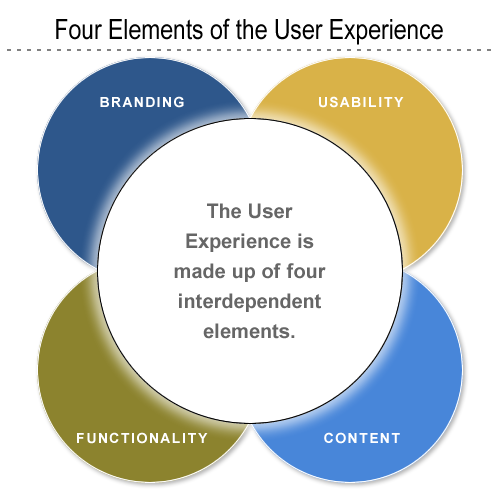
\includegraphics[width=\textwidth]{images/user-experience.png}
	\end{columns}
\end{frame}

\begin{frame}
	\frametitle{用户体验}
	\beamertemplatetransparentcovereddynamicmedium
	\begin{itemize}[<+->]
		\item 用户体验是一个迭代过程,影响用户体验的因素很多:
		\begin{itemize}
			\item 现有技术上的限制\\{\tiny 设计人员必须优先在相对固定的UI框架内进行设计;}
			\item 设计的创新\\{\tiny 在用户的接受程度上也存在一定的风险;}
			\item 开发进度表\\{\tiny 也会给这样一种具有艺术性的工作带来压力;}
			\item 设计人员很容易认为他们了解用户需要\\{\tiny 但实际情况常常不是这样。}
		\end{itemize}
	\end{itemize}
\end{frame}

\begin{frame}
	\frametitle{用户的区别}
	\beamertemplatetransparentcovereddynamicmedium
	\begin{itemize}[<+->]
		\item 用户的分类
		\begin{enumerate}
			\item 偶然型用户\\{\tiny 既没有计算机应用领域的专业知识,也缺少计算机系统基本知识的用户。}
			\item 生疏型用户\\{\tiny 他们更常使用计算机系统,因而对计算机的性能及操作使用,已经有一定程度的理解和经验。但他们往往对新使用的计算机系统缺乏了解,不太熟悉,因此对新系统而言,他们仍旧是生疏用户。}
			\item 熟练型用户\\{\tiny 这类用户一般是专业技术人员,他们对需要计算机完成的工作任务有清楚地了解,对计算机系统也有相当多的知识和经验,并且能熟练地操作、使用。}
			\item 专家型用户\\{\tiny 对需要计算机完成的工作任务和计算机系统都很精通的,通常是计算机专业用户,称为专家型用户。}
		\end{enumerate}
	\end{itemize}
\end{frame}

\begin{frame}
	\frametitle{用户的区别}
	\beamertemplatetransparentcovereddynamicmedium
	\begin{itemize}[<+->]
		\item 计算机领域经验和问题领域经验的区别
		\begin{enumerate}
			\item 用户界面还必须至少从两个维度迎合潜在的广泛经验,这两个维度指的是计算机经验和领域经验。
			\item 计算机经验不仅包括对计算机的一般性了解,还包括对尚待开发的系统的经验。
		\end{enumerate}
		\item 很明显:计算机领域和问题领域经验都不足的用户所需的用户界面与专家用户的界面将区别很大。
	\end{itemize}
	\begin{center}
	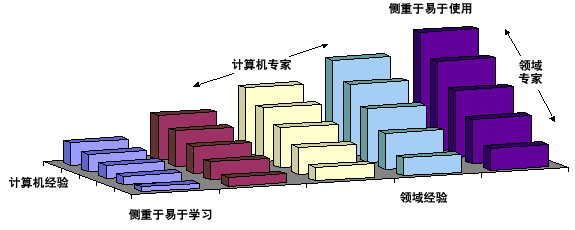
\includegraphics[width=.7\textwidth]{images/user-experts.png}
	\end{center}
\end{frame}

\begin{frame}
	\frametitle{用户交互分析}
	\beamertemplatetransparentcovereddynamicmedium
	\begin{itemize}
		\item 产品策略分析
		\begin{itemize}
			\item 确定产品的设计方向和预期目标\\{\tiny 了解用户对设计产品的期望是什么}
			\item 分析同类型产品的竞争特点\\{\tiny 用户使用同类型产品时的交互体验,包括正面的体验和负面的体验,从而得出产品交互设计的策略。}
		\end{itemize}
		\pause
		\item 用户分析
		\begin{itemize}
			\item 深入而明确的了解产品的目标用户\\{\tiny 特定年龄区间、特殊的文化背景、职业特征、计算机使用经验、同类产品使用经验 \dots}
			\item 找到典型用户。
		\end{itemize}
		\pause
		\item 用户交互特性分析
		\begin{itemize}
			\item 交互挖掘目标用户群,得出准确、具体的用户特征,针对其开展设计。
		\end{itemize}
	\end{itemize}
\end{frame}

\subsection{设计流程}
\begin{frame}
	\frametitle{设计流程}
	\beamertemplatetransparentcovereddynamicmedium
	\tikzstyle{block} = [
		rectangle,
		rounded corners,
		draw=black, very thick,
		fill=blue!20,
		text width=8em,
		minimum height=2em,
		text centered]
	\tikzstyle{line} = [
		draw, -latex',
		draw=black, very thick,
		text centered]

	\begin{columns}
	\column{.5\textwidth}
	\begin{center}
	\begin{tikzpicture}[node distance=1.5cm, auto,]
		\node[block] (a) {用户的观察和分析};
		\uncover<2->{
			\node[block, below of = a] (b) {设计};
			\path[line]	(a)--(b);
		}
		\uncover<3->{
			\node[block, below of = b] (c) {实施};
			\path[line]	(b)--(c);
		}
	\end{tikzpicture}
	\end{center}
	\column{.5\textwidth}
	\begin{itemize}
		\item 用户的观察和分析\\{\tiny 观察用户是如何理解内容和组织信息,指导更合理的设计。}
		\uncover<2->{\item 设计\\{\tiny 将用户分析的结果按讨论对象分类整理,抽象化描述属性、行为、关系。}}
		\uncover<3->{\item 实施\\{\tiny 调整高真 High-fidelity 设计原型,产品设计标准化。}}
	\end{itemize}
	\end{columns}
\end{frame}

\begin{frame}
	\frametitle{用户的观察和分析}
	\begin{itemize}
		\item 情境访谈 Contextual Interviews\\{\tiny 走进用户的现实环境,尽量了解你的用户的工作方式、生活环境等情况。}
		\item 焦点小组 Focus Groups\\{\tiny 组织一组用户进行讨论,让你更了解用户的理解、想法、态度和需求。}
		\item 单独访谈 Individual Interviews\\{\tiny 一对一的用户讨论,让你了解某个用户是如何工作,使你知道用户的感受、想要什么及其经历等。}
	\end{itemize}
\end{frame}

\begin{frame}
	\frametitle{设计}
	\begin{itemize}
		\item 对象模型化\\{\tiny 将用户分析的结果按照讨论的对象进行分类整理,并且以各种图示的方法描述其属性、行为和关系。}
		\item 低真视图 Low-fidelity Prototype\\{\tiny 比较抽象的视图有利于进行逻辑分析。}
		\item 高真视图 High-fidelity Prototype\\{\tiny 比较具体的视图更接近于人机界面的最终表达。}
	\end{itemize}
\end{frame}

\begin{frame}
	\frametitle{实施}
	\begin{itemize}
		\item 设计师对高真设计原型进行最后的调整,并且撰写产品的设计风格标准 Style Guide ,产品各个部分风格的一致性由该标准保证。
		\item 产品实施或投入市场后,面向用户的设计并没有结束,而是要进一步的搜集用户的评价和建议,以利于下一代产品的开发和研制。
	\end{itemize}
\end{frame}

\subsection{任务分析}
\begin{frame}
	\frametitle{任务分析}
	\begin{itemize}
		\item 在以用户为中心的设计中,关心的是如何从用户那里理解和获取用户的思维模式,进行充分、直观的表达,并用于交互设计。
		\item 描述用户行为的工具
		\begin{itemize}
			\item 如通用标识语言 Unified Markup Language, UML~\cite{bjerkander2003architecting}
			\item UML 2.0共有10种图示\\{\tiny 组合结构图、用例图、类图、序列图、对象图、协作图、状态图、活动图、组件图和部署图}
			\item 用以清晰表达一个交互任务诸多方面的内容\\{\tiny 包括交互中的使用行为、交互顺序、协作关系、工序约束 \dots} % 在任务分析中使用UML工具,可以
		\end{itemize}
	\end{itemize}
\end{frame}

\begin{frame}
	\frametitle{任务分析~{\small UML的图示}}
	\begin{tiny}
	\begin{tabular}{|p{.2\textwidth}|p{.4\textwidth}|p{.2\textwidth}|}
	\hline 
	名称 & 视图 & 主要符号 \\ 
	\hline 
	组合结构图 composite-structure diagram & 结构(架构)性需求,主要包括Part、Port、接口和链接(Link) & Part、Port、接口、链接关系 \\ 
	\hline 
	用例图 use case diagram & 功能需求,主要包括用例和参与者 & 用例、参与者、关联关系 \\ 
	\hline 
	类图 class diagram & 静态结构,主要包括一群类及其间的静态关系 & 类、关联关系、泛化关系 \\ 
	\hline 
	序列图 sequence diagram & 一群对象依序传送消息的交互状况 & 对象、消息、活动期 \\ 
	\hline 
	对象图 object diagram & 某时刻下的数据结构,主要包括一群对象及其间拥有的数据数值 & 对象、链接、消息 \\ 
	\hline 
	协作图 collaboration diagram & 一群有链接的对象传送消息的交互状况 & 对象、链接 \\ 
	\hline 
	状态图 state chart diagram & 某种对象的行为,主要呈现一堆状态因事件而转换的状况 & 状态、事件、转换、动作 \\ 
	\hline 
	活动图 activity diagram & 一段自动转换的活动流程,主要包括一堆活动及其间的自动转换线 & 活动、转换、分叉、接合 \\ 
	\hline 
	组件图 component diagram & 一群组件及其间的依赖关系 & 组件、接口、依赖关系、实现关系 \\ 
	\hline 
	部署图 deployment diagram & 一堆设备及其间的依赖关系 & 节点、组件、依赖关系 \\ 
	\hline 
	\end{tabular} 
	\end{tiny}
\end{frame}

\begin{frame}
	\frametitle{例~{\small 图书馆管理系统}}
	从读者提出想要借书开始,经过如下五个交互步骤:
	\begin{enumerate}
		\item 根据系统提供查询功能,读者可以在系统界面中输入关键字查询图书;
		\item 系统通过交互界面列出可借用的图书供读者选择;
		\item 如果读者选定了图书,系统提示读者输入借书证号和密码;
		\item 如果最后读者确定借阅关系,系统处理并通知读者借书成功,并给读者一个确认;
		\item 当确认信息出现时,整个图书借阅的交互过程就结束了。
	\end{enumerate}
\end{frame}

\begin{frame}
	\frametitle{例~{\small 任务分析内容}}
	\beamertemplatetransparentcovereddynamicmedium
	\begin{itemize}[<+->]
		\item 使用行为分析~{\tiny 哪些人、哪些事?}
		\item 顺序分析~{\tiny 什么流程?}
		\item 协作关系分析~{\tiny 怎么配合?}
		\item 工序约束分析~{\tiny 依赖关系?}
		\item 用户任务总览
		\item 任务层次关系~{\tiny 子任务划分}
		\item 故事讲述和情节分析~{\tiny 应用场景重现}
	\end{itemize}
\end{frame}

\begin{frame}
	\frametitle{例~{\small 使用行为分析}}
	\beamertemplatetransparentcovereddynamicmedium
	\begin{itemize}
		\item 理解系统中每个参与者及其所需完成的任务,即
		\begin{itemize}
			\item 分析系统所涉及的问题领域和系统运行的主要任务
			\item 分析使用该系统主要功能部分的是哪些人,谁将需要该系统的支持以完成其工作。
		\end{itemize}
		\pause
		\item 一般使用用例图描述\\{\tiny 从参与者的角度出发来描述一个系统的功能,主要目的是帮助开发团队以一种可视化的方式理解系统的功能需求。}
		\pause
		\item 图书馆管理系统用户主要包括
		\begin{itemize}
			\item 读者(借阅者)
			\item 图书管理员
			\item 图书馆管理系统的系统管理员
		\end{itemize}
	\end{itemize}
\end{frame}

\begin{frame}
	\frametitle{例~{\small 读者请求服务用例}}
	\includegraphics[width=\textwidth]{images/lib-reader-use-case.pdf} 
\end{frame}

\begin{frame}
	\frametitle{例~{\small 图书管理员处理借、还书用例}}
	\includegraphics[width=\textwidth]{images/lib-manager-use-case.pdf} 
\end{frame}

\begin{frame}
	\frametitle{例~{\small 系统管理员维护系统用例}}
	\includegraphics[width=\textwidth]{images/lib-admin-use-case.pdf} 
\end{frame}

\begin{frame}
	\frametitle{例~{\small 顺序分析}}
	\beamertemplatetransparentcovereddynamicmedium
	\begin{itemize}
		\item 每个使用行为都是由若干步骤组成的,这些步骤可以使用顺序图进行描述。
		\begin{itemize}[<+->]
			\item 顺序图描述了完成一个任务的典型步骤;
			\item 可以按照交互任务发生的时间顺序,把用例表达的需求转化为进一步、更加正式层次的精细表达;
			\item 用例常常被细化为一个或更多的顺序图。
		\end{itemize}
	\end{itemize}
\end{frame}

\begin{frame}
	\frametitle{例~{\small 读者借书时序图}}
	\includegraphics[width=\textwidth]{images/lib-reader-borrow-sequence.pdf} 
\end{frame}

\begin{frame}
	\frametitle{例~{\small 协作关系分析}}
	\beamertemplatetransparentcovereddynamicmedium
	\begin{itemize}[<+->]
		\item 协作图
		\begin{itemize}
			\item 着重显示某个用户行为中各个系统元素之间的关系,不再重点强调各个步骤的时间顺序。
		\end{itemize}
	\end{itemize}
\end{frame}

\begin{frame}
	\frametitle{例~{\small 协作关系分析图}}
	\includegraphics[width=\textwidth]{images/lib-user-relationship.pdf} 
\end{frame}

\begin{frame}
	\frametitle{例~{\small 工序约束陈述}}
	\beamertemplatetransparentcovereddynamicmedium
	\begin{itemize}[<+->]
		\item 用户完成任务的步骤又被称为工序
		\begin{itemize}
			\item 某些工序之间的顺序有逻辑关系
			\item 工序约束陈述是工序分析的最直接的方法
		\end{itemize}
		\item 图书管理系统通常存在如下工序约束:
		\begin{itemize}
			\item 系统管理员必须先增加借阅者信息,读者才能登陆。
			\item 系统管理员必须先增加书籍信息,读者才能查阅。
			\item 读者借阅信息生成后,图书管理员图书管理员才能去书库取书。
			\item 读者必须先在系统中办理借阅,才能取书。
			\item 读者必须先借书才能还书。
		\end{itemize}
	\end{itemize}
\end{frame}

\begin{frame}
	\frametitle{例~{\small 用户任务一览表}}
	\begin{itemize}
		\item 所有任务分析完毕后即可用一览表的形式描述系统中的所有用户及其可能需要完成的所有任务
		\begin{itemize}
			\item 一目了然的展示所有用户的交互任务信息,并且便于更改和调整。
		\end{itemize}
	\end{itemize}
	\begin{center}
	\begin{tiny}
	\begin{tabular}{|l|c|c|c|}
	\hline 
	任务 & 读者 & 图书馆管理员 & 系统管理员 \\ 
	\hline 
	书籍信息查询、读者信息查询 & √ & √ & • \\ 
	\hline 
	借书 & √ & √ & • \\ 
	\hline 
	还书 & √ & √ & • \\ 
	\hline 
	书籍预定 & √ & √ & • \\ 
	\hline 
	增加、删除或更新书目 & • & • & √ \\ 
	\hline 
	增加、删除书籍 & • & • & √ \\ 
	\hline 
	增加、删除或更新读者帐户信息 & • & • & √ \\ 
	\hline 
	\end{tabular} 
	\end{tiny}
	\end{center}
\end{frame}
 
\begin{frame}
	\frametitle{例~{\small 协作关系分析图}}
	\includegraphics[width=\textwidth]{images/lib-user-relationship.pdf}
\end{frame}

\begin{frame}
	\frametitle{例~{\small 任务金字塔}}
	\begin{itemize}
		\item 描述不同层次任务之间的关系
		\begin{itemize}
			\item 任何一个任务都可能包括若干子任务,从而构成金字塔状的结构。
			\item 本例中,读者查询图书:
		\end{itemize}
	\end{itemize}
	\begin{center}
	\includegraphics[width=.8\textwidth]{images/lib-reader-query.pdf}
	\end{center}
\end{frame}

\begin{frame}
	\frametitle{故事讲述和情节分析}
	\beamertemplatetransparentcovereddynamicmedium
	\begin{itemize}
		\item 描述实际的任务场景
		\begin{itemize}
			\item 直观说明任务,便于与用户交流
			\item 帮助分析设计者和真正用户之间对任务的不同理解
		\end{itemize}
		\pause
		\item 故事讲述 story telling 可真实或虚构
		\begin{itemize}
			\item 可为对理想场景或极端情况
			\item 关键在于充分的代表性,可典型的反映交互任务。
		\end{itemize}
		\pause
		\item 情节分析 scenario analysis 是对故事所反映的交互任务的理性分析
		\begin{itemize}
			\item 分离出故事中所描述的角色、目标、环境、步骤、策略、感情等诸方面的因素。
		\end{itemize}
		\pause
		\item 作为任务分析的基础,系统设计的依据,系统评估的工具。 % 测试案例
	\end{itemize}
\end{frame}

\begin{frame}
	\frametitle{例~{\small 图书馆典型交互}}
	\begin{itemize}
		\item 故事:学生借书过程中与图书馆系统交互
		\begin{itemize}
			\item 角色:刘凡,图书馆读者;图书管理员。
			\item 目标:完成书籍的借阅或预定。
			\item 环境:图书馆借阅大厅,有查询电脑可供查询使用;借书处,取到借阅的书籍。
			\item 步骤:查询书籍,浏览图书信息,确定要借阅的书籍;然后在系统中办理借阅,并等待从借书处取书。
			\item 策略:如果图书在馆,则借阅;否则,可以预定图书。
			\item 情感:交互系统的交互过程简洁、顺畅,信息提示充分、清晰,用户对完成任务的过程感到满意。
		\end{itemize}
	\end{itemize}
\end{frame}

%\subsection{以用户为中心的界面设计}
%\begin{frame}
%	\frametitle{以用户为中心的界面设计}
%
%\end{frame}

\section{小结}
\begin{frame}
	\frametitle{小结}
	\begin{itemize}
		\item 理解人机界面设计的一般原则
		\item 掌握以用户为中心的界面设计方法
	\end{itemize}
\end{frame}

\begin{frame}
	\frametitle{参考文献}
	\bibliographystyle{plain}
	\bibliography{hci}
\end{frame}

\end{document}